\documentclass[a4paper,17pt]{article}

% Language setting
\usepackage[english]{babel}
\usepackage{algorithm} 
\usepackage{algpseudocode} 

% Set page size and margins
\usepackage[a4paper,top=2cm,bottom=2cm,left=3cm,right=3cm,marginparwidth=1.75cm]{geometry}

% Useful packages
\usepackage{amsmath}
\usepackage{graphicx}
\usepackage[colorlinks=true, allcolors=blue]{hyperref}

\title{Rectilinear Partitioning of Rectilinear Polygon using Dynamic Programming}
\author{Dibyendu Saha, M.Tech, University Of Kalyani\linebreak}
\date{}
\begin{document}
\maketitle

\begin{abstract}
In this paper we propose an algorithm for partitioning a rectilinear polygon into a minimum number of rectangles using a minimum number of cut lines using dynamic programming. We take the input points, possible cut lines, and possible points that cut the existing edges on new points and we will also take the intersection points of each cut line and we take each possible combination from these set of points into consideration to create the rectangles and to find the optimal result. We tried to make the algorithm to find the optimal cuts we can have on the input polygon that will divide the polygon in n sub rectangles. This algorithm will take the orthogonal hull points of the polygon as an input and it will give output as a set of optimal rectangles it finds. 
\end{abstract}

\section{Introduction}

Partitioning complex Polygons is the fundamental problem in digital geometry and it helps to identify the similar features between multiple building plans, load distribution, chip manufacturing, pattern recognition and Geo-informatics. The first time this problem arose because of the growing VLSI layout design image processing industries due to their real world applications. In this paper we will propose an algorithm to partition an rectilinear polygon using multiple rectilinear rectangles with the main objective to minimise the number of rectangles and cuts we need to have to create those polygons. 

\vspace{5mm} %5mm vertical space

\begin{figure}[!h]
\centering
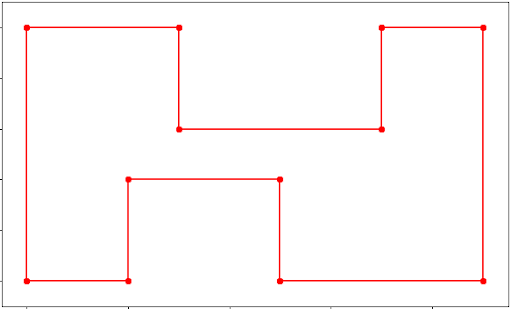
\includegraphics[width=1\textwidth]{input-rectilinear-polygon.png}
\caption{Input Rectilinear polygon}
\label{fig:IRP}
\end{figure}

If we try to solve this problem using our human eye, the first thing we do is to find a rectangle that will consume the maximum area, and we repeat the process with leftover area until the whole area is covered. If any area is left and requires more rectangles we adjust the first rectangle and repeat the process once more time. This is the exact thing we implement in our algorithm. 
We will try to find the minimum rectangle by trying to maximise the area of each rectangle we find so that each rectangle will consume the maximum area of any given polygon figure [\ref{fig:IRP}] and the number of rectangles will be minimum. By finding the minimum number of rectangles we can also find the cut lines that will be needed to make the number of rectangles minimum by comparing and merging the edges of the new sub rectangles with the given hull edges. The new lines that will not be in the input hull will be our optimal cuts.  In this kind of rectilinear partitioning some rectangles will have one or more of the rectilinear polygon points taken from initial orthogonal hull points as per work of Hwi Kim\cite{https://doi.org/10.48550/arxiv.2111.01970}. 

\begin{figure}[!h]
\centering
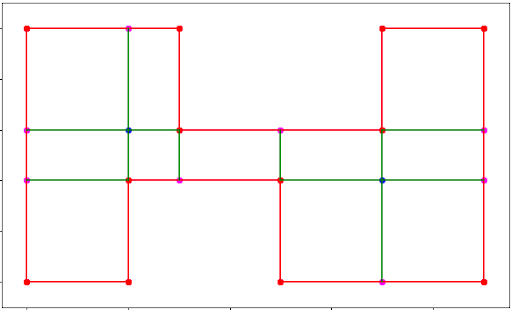
\includegraphics[width=1\textwidth]{points-marked.png}
\caption{Points marking; 1.red vertices are the initial points, 2. Red lines are the initial rectilinear polygon lines, 3. Green lines are the cut lines by extending initial points, 4. Pink points are the projection points of the cut lines, 5. Blue points are the intersection points of the initial cut lines.}
\label{fig:PM}
\end{figure}

We will try to create rectangles from each corner point and so there will be horizontal and vertical lines intersecting the whole polygon and landing on other edges. These new edge points will be placed to the set of orthogonal hull points too and this will be our new set of hull points. We will also calculate the intersection points of two or more cut lines and now the set of the new hull points and intersection points will be passed as an input to the greedy algorithm. The points are shown in \figureautorefname[\ref{fig:PM}]

Now the algorithm will compute the possible combination of 4 points among the new ponts set, and each possible rectangle will be processed to decide whether it is allowed to be a possible sub-rectangle or not. If it is eligible to be a rectangle we will compare it with the maximum area, if it's more than the previous maximum area, we will restart the process starting with this rectangle. After we found the eligible candidates we will then perform merging by taking each possible combination of rectangle set and merging two or more rectangle with fall to one, of there is an overlap and union of those two rectangle does not form a rectangle we will cut the portion of smaller rectangle to resolve it. After we got the final rectangle set, this needed to be compared with the input hull to find the cut lines to make the rectangles.

\section{Paper Organisation}
We will Start with the methodology we used to build our algorithm. After that we will discuss about the main algorithm and the various parts of it. Next We will summarize the algorithm and Later We will take few example rectilinear polygon and discuss the results of of our algorithm on those examples. Then we have a brief look on the future scope of this algorithm, and we will end our paper with conclusion and references.

\section{Methodology}
The proposed algorithm consists of the following steps; 1. At first we find the orthogonal hull of the given polygon object. Then we extend each hull point internally within the polygon to find the cut points that fall on other edges. We also compute the intersection points of line cut points. 2. Next we will take the union of a set of points of initial hull point, cut point on each edge and cut intersection points and we will try to compute each possible rectangle combination that falls within the input polygon and create a set of possible rectangles. 3. And at last we combine the rectangle in such a way that there is no overlap between any rectangle, no portion of any rectangle is not outside of the hull, total area of the given hull is covered and the number of rectangles is minimum.

\section{Algorithm Description}
Our algorithm has three parts: points marking, sub rectangle calculation, and then merging the rectangles. 

\subsection{Points Marking} \label{sec:point-marking}
In this algorithm we will first try to find potential candidates of the optimal rectangle solution. There are three types of candidate points, initial candidates those who are on the orthogonal hull, projection points that fall on any edge of the hull and the intersection points of the projection lines. Then these potential points are feed-ed into the rectangle creation part.

\subsubsection{Initial Points}
Initial points are the given input orthogonal hull points. We will start from these initial points and try to find other potential points for the optimal rectangles. This points are the corner points of each hull so we can assume there will be one or more react-angle for each hull corner point.
\subsubsection{Projection Points}
On any orthogonal hull if we want to divide it into multiple pieces we need to goto each edges one by one and need to check if there exist a perpendicular on that line passing through any hull points in a way there is no part of the cut line exist outside the given polygon this new point is the projection point, this projection point needs to be inline with the two vertices of the edge. As this projection point is on the edge we need to make sure this projection point is not any vertex of the initial point and the projection line or cut line is not an edge. If the projection point passed all the above criteria we will add the projection point into the initial hull points.


\begin{algorithm}
    \caption{Pseudo code for generating projection points}
	\label{alg:GPP}
    \begin{algorithmic}[1]
	    \Procedure{$generateProjectionPoint$}{$polygon$}
            \Comment{$INPUT : Rectilinear Polygon$}
    	    \State $points \leftarrow getPointsFromPolygon(polygon)$
    	    \State $edges \leftarrow getEdgesFromPolygon(polygon)$
    	    \State $cutLines \leftarrow []$
    	    \For {$ each \ p \in points, \ldots$}
        	    \For {$ each \ edge \in edges, \ldots$}
    	            \State $projectionPoint \leftarrow getProjectionPoint(edge,\ point)$
    	            \If {$(edge[0],\ projectionPoint\ and\ edge[1]\ are\ in\ same\ line) \And (projectionPoint\ is\ not\ edge[0]\ or\ edge[1])$}
    	                \State $cut \leftarrow [point, projectionPoint]$
    	                \If {$(point\ is\ not\ projectionPoint) \And (cut\ not\ in\ edges) \And (cut\ not\ fall\ outside\ the\ polygon) \And (projectionPoint\ not\ in\ points)$}
    	                    \State {$insert projectionPoint into points after index of edge[0]$}
    	                    \State {$cutLines.append(cut)$}
    	                \EndIf
    	            \EndIf
    			\EndFor
    		\EndFor
		\EndProcedure
	\end{algorithmic}
\end{algorithm}

these are the sub algorithms we use to in order to get the Algorithm [\ref{alg:GPP}]. These all are the helper function of the Algorithm [\ref{alg:GPP}].

Algorithm [\ref{alg:FPP}] is to generate a list of points from a polygon object.

\begin{algorithm}
    \caption{Pseudo code for finding polygon points}
    \label{alg:FPP}
    \begin{algorithmic}[1]
        \Procedure{$getPointsFromPolygon$}{$polygon$}
            \State {$points \leftarrow makeIterableArrayOfPoints(polygon)$}
            \State \Return {$points$}
        \EndProcedure
    \end{algorithmic}
\end{algorithm}

Algorithm [\ref{alg:FPE}] is to generate a list of edges from a polygon object.

\begin{algorithm}
    \caption{Pseudo code for finding polygon edges}
    \label{alg:FPE}
    \begin{algorithmic}[1]
        \Procedure{$getEdgesFromPolygon$}{$polygon$}
            \State {$index \leftarrow 0$}
            \State {$points \leftarrow getPointsFromPolygon(polygon)$}
            \State {$pointsCount \leftarrow points.length$}
            \State {$edges \leftarrow []$}
            \For{$index < pointsCount \ldots $}
                \State {$line = [points[index], points[mod(index+1, pointsCount-1) ] $}
                \State {$edges.push(line)$}
                \State {$index \leftarrow index+2$}
            \EndFor
            \State \Return{$edges$}
        \EndProcedure
    \end{algorithmic}
\end{algorithm}

Algorithm [\ref{alg:FSPP}] is to single projection point of a point to a edge.

\begin{algorithm}
    \caption{Pseudo code for finding single projection point}
    \label{alg:FSPP}
    \begin{algorithmic}[1]
        \Procedure{$getProjectionPoint$}{$edge,\ p$}
	        \State {$x \leftarrow edge[0]$}
            \State {$y \leftarrow edge[1]$}
            \State {$x1, y1 \leftarrow x[0], x[1]$}
            \State {$x2, y2 \leftarrow y[0], y[1]$}
            \State {$xp, yp \leftarrow p[0], p[1]$}
            \State {$x12 \leftarrow x2 - x1$}
            \State {$y12 \leftarrow y2 - y1$}
            \State {$dotp \leftarrow x12 * (xp - x1) + y12 * (yp - y1)$}
            \State {$dot12 \leftarrow x12 * x12 + y12 * y12$}
            \If{$dot12 == True$} 
                \State {$ coeff \leftarrow dotp / dot12 $}
                \State {$ lx \leftarrow x1 + x12 * coeff $}
                \State {$ ly \leftarrow y1 + y12 * coeff $}
                \State {$ \Return (int(lx), int(ly)) $}
            \Else
                \State \Return {$False$}
            \EndIf 
            \EndProcedure
    \end{algorithmic}
\end{algorithm}

After we find the projection points those points need to be inserted into proper places in the points array so that we can loop though the new points one by one. 

\subsubsection{Intersection Points}
The main target is to collect maximum number of possible potential points that will become part of optimal rectangle. After we find the intersection lines we need to compute the intersection point of the cut lines as this points will be also potential points to form the optimal rectangles. We will also consider multiple points from the same cut line if there exist more overlap. this will be last step to generate potential points. To find the intersection points the pseudo code is described in Algorithm [\ref{alg:FIP}]


\begin{algorithm}
    \caption{Pseudo code for finding Intersection points}
    \label{alg:FIP}
    \begin{algorithmic}[1]
        \Procedure{$generateIntersectionPoint$}{$cutLines$}
    	\Comment{$Input: cutLines$}
        \State {$intersections \leftarrow []$}
        \For {$each\ line1 \in cutLines \dots$}
            \For {$each\ line2 \in cutLines \dots$}
                \If {$(line1 == line2) \And (line1[0]==line2[0]) || (line1[0]==line2[1]) || (line1[1]==line2[0]) || (line1[1]==line2[1])$}
                    \State {\bf continue}
                \EndIf
                \State {$intersectionPoint \leftarrow lineIntersection(line1, line2)$}
                \If {$(intersectionPoint is not Null) \And (intersectionPoint not in intersections) \And (intersectionPoint not in new_points)$}
                    \State {$intersections.append(intersectionPoint)$}
                \EndIf
            \EndFor
        \EndFor
        \State \Return {$intersections$}
	\EndProcedure
    \end{algorithmic}
\end{algorithm}


After finding all of the above points we will create the set by taking union of it. All types of points are shown in Figure [\ref{fig:PM}]. Pink points are the projection points, blue points are the intersection points and green lines are the projection line from initial hull point to projection point.


\subsection{Sub Rectangle Calculation}
On this step we will perform dynamic programming to find all types of of rectangular polygon that can be formed by the points set got from section \ref{sec:point-marking}. We will take any four points form the point set and we will check if its a rectangle and eligible to be a potential rectangle or not.
\begin{figure}[h]
\centering
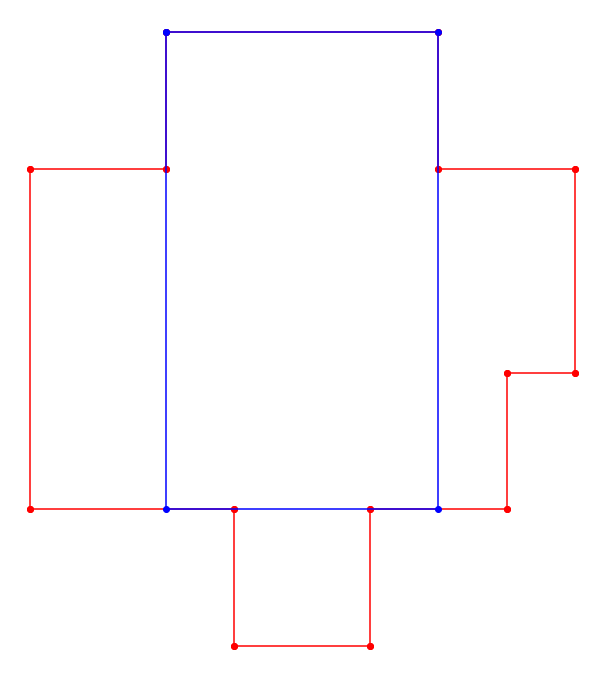
\includegraphics[width=0.67\textwidth]{max-area.png}
\caption{Capturing the rectangle having the the max\_area }
\label{fig:MA}
\end{figure}
Also by this algorithm we will try to fit the maximum possible rectangle on to this polygon. To find this we will start with a rectangle that has the maximum area among other rectangle until now. If we found any point set(rectangle) that has the area more than the $max\_area$ we will start over the process with this rectangle as the starting point.
\newline
Rectangle finding function will take three arguments as input set of all points, {$max\_area$} found till now, vertices of the {$max\_rectangle$} and the primary polygon. Now we need to take the permutation combinations of all points to take 4 points {$nP4$}. We need to check if the taken 4 points are the valid rectangle or not.  We can easily do so by drawing a bounding box rectangle of these 4 points by calculating {$min\_x, min\_y; max\_x, min\_y,\ max\_x,max\_y\ and\ min\_x,\ max\_y$}. And then check if the area of the bounding box is the same as the area of the taken points polygon and there are no two lines of these 4 points in the same line. We also need to test if the intersection area of this polygon and primary polygon is zero. the area of this rectangle is less than the max\_area we found as the argument. If we found any case where the new rectangle area is more, the function will return this rectangle back, and we need to start over the permutation again so that we will start from the beginning. The main objective of doing this is to find the rectangle having the maximum area and then making the smaller rectangle so that there will be less number of rectangles to be processed in the merging function. After these test cases if passed we again need to check whether any form of these four rectangles is already interested into the new rectangle set if not insert it to the final\_set. After all the permutation ends, return the final set. The final set is shown in Figure[\ref{fig:FO}]


\begin{algorithm}
    \caption{Pseudo code for finding sub rectangles}
    \label{alg:FSR}
    \begin{algorithmic}[1]
    \Procedure{$findRetangles$}{$allPoints,\ rectangles,\ max\_area,\ primaryPoly$}
        \For{$each\ poly \in permutation(all\_points,\ 4)$}
            \If {$(poly.area\ \neq 0) \And ( poly.area == enclosed_rectangle(poly) ) \And (poly \notin rectangles)$}
                \State {$allowd\_to\_add \leftarrow False$}
                \If {$rectangles.length == 0$} 
                    \State {$allowd\_to\_add \leftarrow True$}
                \Else
                    \State {$has\_overlap \leftarrow False$}
                    \For {$each\ \in rectangles$}
                        \If {$hasOverlap(poly, rect)$}
                            \State {$has\_overlap = True$}
                            \State {$\bf break$}
                        \EndIf
                    \EndFor
                    \If {$has\_overlap == False$}
                        \State {$allowd\_to\_add \leftarrow True$}
                    \EndIf
                    \If {$allowd\_to\_add \And primary\_poly.intersection(poly).is\_closed\_area$}
                        \If {$poly.area > max_area$}
                            \State \Return [poly], True, poly.area
                        \EndIf
                        \State {$rectangles.append(poly)$}
                    \EndIf
                \EndIf
            \EndIf
        \EndFor
        \State \Return {$rectangles, False, max_area$}
    \EndProcedure
    \end{algorithmic}
\end{algorithm}



\begin{figure}[h]
\centering
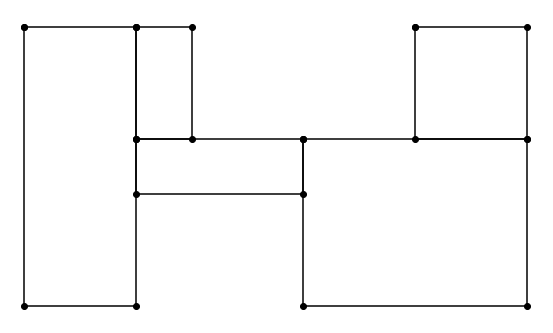
\includegraphics[width=1\textwidth]{final-output.png}
\caption{Valid  sub rectangles from new points by rectangle generation algorithm.}
\label{fig:FO}
\end{figure}

\bibliographystyle{unsrt}

% \addbibresource{references.bib}
% \printbibliography

% \printbibliography
\bibliography{references}


\end{document}